\chapter{Erweiterte Funktionen}
In diesem Kapitel werden nun weitere Funktionen beschrieben, die über die Grundausstattung der Web-App und die WebSockets hinausgehen, um die Arbeit zu erweitern und produktiver zu gestalten. 

%%%%%%%%%%%%%%%%%%%%%%%%%%%%%%%%%%%%%%%%%%%%%%%%%%

\section{Entwurfsmuster: Publish / Subscribe}
Mit Publish / Subscribe (deutsch: veröffentlichen / abonnieren) wird ein Muster beschrieben, mit dem ein Client eine Benachrichtigung erhält, sofern ein Ereignis verändert wurde, welches von ihm abonniert wurde. Bei diesem Entwurfsmuster wissen weder Publisher noch Subscriber voneinander und es läuft vollkommen unabhängig, asynchron miteinander. Sie müssen auch nichts voneinander wissen, da sämtlicher Datenaustausch über den socket.io Server läuft \cite{autobahn.js:pubsub}.\par

Konkret können in dieser Anwendung Veranstaltungen abonniert werden. Das geschieht automatisch über die Webanwendung selbst, welche dem WebSocket Server mit Einloggen des Benutzers eine subscribe Nachricht schickt. Ausgewählt werden die Events, die der Benutzer selbst erstellt hat. 

Gab es eine Änderung an einer Veranstaltung, so meldet sich die Web-App beim WebSocket Server mit einer \emph{publish}-Nachricht. Dieser schaut dann in seiner Liste der authentifizierten Clients nach, welcher die Veranstaltung abonniert hat und schickt an alle verbundenen Endgeräte eine Mitteilung, dass die Veranstaltung bearbeitet wurde.\par

\paragraph{Implementierung}
Im ersten Entwurf der Technik in dieser Arbeit wurden alle Nachrichten, die über WebSockets verschickt wurden, über die Clients selbst versendet, da die Kommunikation nur über JavaScript nativ unterstützt wird. Daher wurden auf Basis von Elephant.io Methoden entwickelt, die die publish-Funktion der Webanwendung übernehmen.\\
Der EventsController hat nun noch die zusätzliche Aufgabe bei jedem Datenbankzugriff eine Verbindung zum WS Server zu öffnen, eine publish-Nachricht abzuschicken, und dann die Verbindung wieder zu schließen.\\
Dadurch funktioniert Publish/Subscribe auch mit Endgeräten, die JavaScript verbieten. Die Clients, die Nachrichten erhalten möchten, bekommen diese nun ungehindert zugestellt.\par

\begin{figure}[!ht]
	\centering
	
\includegraphics[width=15cm]{fig/noty_android}
	\caption{publish-Benachrichtigung am unteren Bildschirmrand mit Android 4.3}
\end{figure}

So ist es nun möglich über WebSockets eine Benachrichtigung an die Abonnenten zu schicken. Dadurch wird man aktiv informiert, wenn Änderungen an den Veranstaltungen vorgenommen werden. 

%%%%%%%%%%%%%%%%%%%%%%%%%%%%%%%%%%%%%%%%%%%%%%%%%%

\section{Lokalisierung von Clients}
Mit HTML5 wurde die \emph{navigator.geolocation} Klasse in die JavaScript API eingebaut. Diese Klasse ermöglicht es einer Webanwendung die Position des Anwenders zu erhalten - aber nur, wenn der Anwender zustimmt. Das geschieht mittels in der Umgebung befindlichen W-Lan Netzwerke, der eigenen IP und wird dann mit einem Google Service abgeglichen. Verfügt das Gerät über GPS, so werden diese Daten auch berücksichtigt und ermöglichen eine genauere Ortung \cite[1. Absatz]{html5:geolocations}.

\paragraph{Koordinieren von Helfern}
Um die eingetragenen Helfer in dieser Webanwendung besser koordinieren zu können, wurde daher ein Skript implementiert, welches im Hintergrund der Web-App läuft und die aktuelle Position des Endgeräts über eine SSL verschlüsselte Verbindung an den Server übermittelt. Unter der Voraussetzung, dass der Client diesem Vorgang zustimmt sind dem Server damit die Positionen der eingeloggten Benutzer bekannt. Diese Positionsdaten können dann von der Anwendung ausgewertet und in einer Karte von \emph{Google Maps} \cite{google:maps} visualisiert werden.

\begin{figure}[!ht]
	\centering
	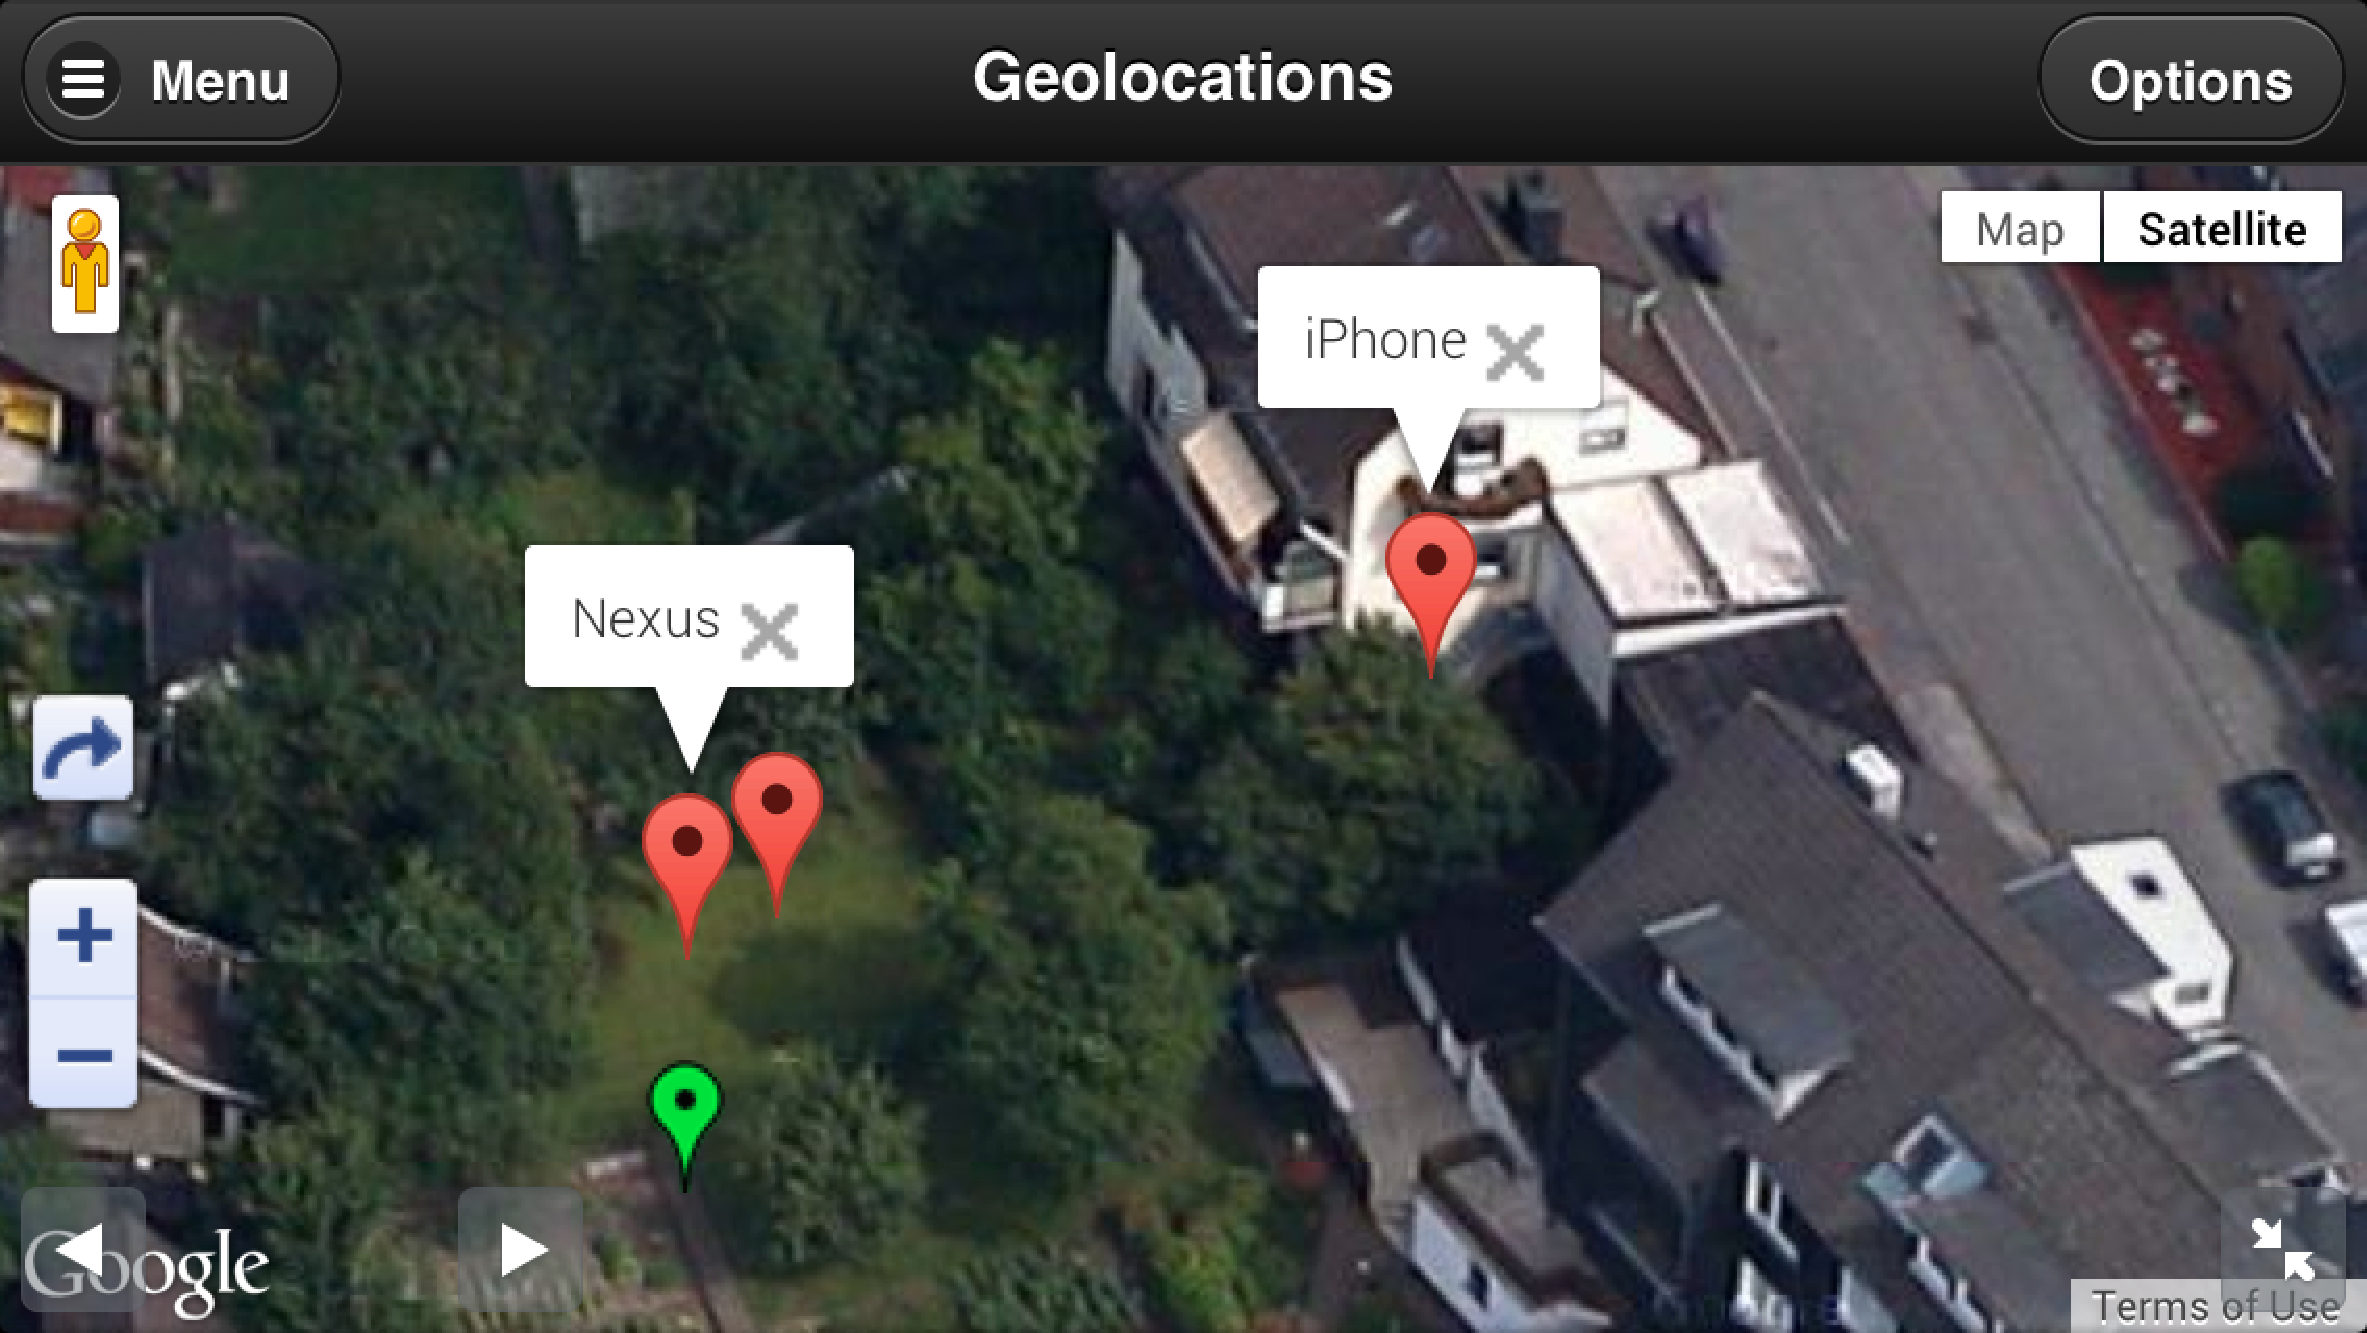
\includegraphics[width=15cm]{fig/screenshot_geolocations}
	\caption[Beispielansicht der Geolocations]{Getestet unter iOS 6.1.4, iPhone 5, Safari: Grün markiert eigene Position. Durch Tippen auf andere Marker erscheint der Name des Benutzers}
\end{figure}

Jeder Client kann auf diese Weise die Positionen der anderen Helfer sehen. Der Vorteil liegt klar auf der Hand: eine zentral eingerichtete Verwaltung kann mit einem Blick sehen, wer sich an welcher Stelle auf dem Gelände befindet. So können Wege optimiert und gezielt Aufgaben an sogenannte Springer verteilt werden, da ortsnahe Helfer die entsprechenden Aufgaben übernehmen können. Die kurzen Wege sorgen dann dafür, dass eine höhere Nutzung der Ressourcen (hier: die Helfer) möglich ist.\par

\paragraph{Anforderungen}
Eine wichtige Anforderung an diese Funktion ist, dass die Daten schnell ausgetauscht werden. Wenn zwischen den Updates der Geolocations zu viel Zeit vergeht, ist die Position nicht mehr aktuell und damit nicht mehr relevant. Deswegen findet der Austausch von Longitude und Latitude auch über WebSockets statt.

\paragraph{Kein Speichern der Positionsdaten}
Beendet ein Client die Verbindung oder erhält der Server keine Aktualisierungen mehr, so wird sein letzter Standort noch 15 Minuten gespeichert und dann auf allen Endgeräten gelöscht. Zu keiner Zeit werden Daten protokolliert oder länger als nötig aufbewahrt.

\subsection{Umgebungsbedingte Einschränkungen}
Bei diesem Projekt handelt es sich um eine Webanwendung, die aufgrund von Sicherheitsvorkehrungen einigen Einschränkungen unterliegt. So erlauben die mobilen Betriebssysteme keine Geopositionierung durch den Browser, wenn dieser minimiert ist oder das Smartphone / Tablet nicht aktiv genutzt wird. Das bedeutet, dass die Meißner App geöffnet sein muss, damit alle Funktionen genutzt und aktualisiert werden können.\par

Das ist für die Lokalisierung problematisch, da so die Position des Clients nicht aktuell bleibt. Diese Sicherheitsmaßnahmen sind jedoch sehr sinnvoll, denn es wäre sehr bedenklich könnte eine Homepage im Hintergrund stetig die Position des Besuchers überwachen. Allerdings genügt es, wenn die Webanwendung in einem Tab geöffnet ist, welcher nicht aktiv sein muss, um die Position des Endgeräts zu erfahren.

%%%%%%%%%%%%%%%%%%%%%%%%%%%%%%%%%%%%%%%%%%%%%%%%%%

\section{Analyse der Skalierbarkeit}
An den Webserver auf Apache-Basis o.Ä. werden mit der Meißner-App keine hohen Anforderungen gestellt, da ressourcenschonend entwickelt wurde und nur wenige SQL-Querys nötig sind für die Anzeige der Views. Interessanter ist allerdings die Echtzeitaktualisierung, da diese mit steigender Anzahl von Endgeräten deutlich mehr Sockets verwalten und mit Updates beliefern muss.

\subsection{Zeitliches vs. konditionelles Update}
Die \emph{navigator.geolocation} Klasse bietet mehrere Möglichkeiten seine Position zu aktualisieren. Jede Option wurde in Erwägung gezogen, die Zugriffe gemessen und schließlich in einer Tabelle ausgewertet. Die Auswertung ist daher interessant, weil die Skalierbarkeit dieser App noch nicht betrachtet wurde.\par

Mit einbauen: http://hacks.mozilla.org/2009/06/geolocation/\par

Die Statistiken hier baue ich noch ein...

%%%%%%%%%%%%%%%%%%%%%%%%%%%%%%%%%%%%%%%%%%%%%%%%%%

\section{Paketierung für App-Stores}
Auch bei Web-Apps besteht die Möglichkeit diese in den gängigen App-Stores wie dem von Apple oder Googles Play Store anzubieten. Dafür gibt es einige Frameworks, welche die eigentliche Webanwendung in eine Browserumgebung verpacken und diese dann wie eine native App aussehen lassen.\par
Für diese Arbeit wurde bewusst nicht darauf eingegangen und auch keine Paketierung für die Stores eingeplant. Das gesamte Projekt soll sehr dynamisch sein und ohne Grenzen der Stores für alle Geräte zur freien Verfügung stehen. Und eine Webseite aufrufen ist da die einfachste Möglichkeit die Anwendung zu nutzen.

\paragraph{Vorteile}
So können Änderungen an der Meißner App vorgenommen werden ohne, dass man kompliziert über die Stores die App neu verteilen muss. Außerdem ist absolut keine Installation notwendig, da sie wie eine normale Homepage geladen wird. Der Benutzer ist zwar nicht zwangsläufig gewohnt Apps über einen anderen Weg als den bekannten Store zu beziehen, aber da die Web-App genau so einfach geöffnet wird wie der Aufruf einer Homepage, kann man davon absehen.

\subsection{Add to Homescreen}
Bei Geräten mit dem Betriebssystem iOS ist die Funktion \emph{Add to Homescreen} verfügbar, welche eine Verknüpfung zur Webanwendung auf dem Homescreen erstellt. So kann die Anwendung wie eine normale App gestartet werden.\\
Durch eine einfache Ergänzung im Header der mobilen HTML Seite wird so eine appähnliche Installation ermöglicht.
\\
\begin{lstlisting}[captionpos=b, caption=Ergänzung im Header der mobilen Seite]
  <meta name="apple-mobile-web-app-capable" content="yes">
  <meta name="apple-mobile-web-app-status-bar-style"
  	content="black">
  <link rel="apple-touch-icon" href="img/icon.png">
\end{lstlisting}
Mit diesen drei Zeilen wird zuerst die Option \emph{Add to Homescreen} erlaubt, dann die Statusleiste schwarz gefärbt und der Pfad zum Icon angegeben, welches dann auf dem Homescreen erscheinen soll.\par

Das stellt eine einfache Möglichkeit dar eine Web-App zu installieren, allerdings gibt es keine ähnliche Funktion unter anderen Betriebssystemen wie Android o.Ä..

%%%%%%%%%%%%%%%%%%%%%%%%%%%%%%%%%%%%%%%%%%%%%%%%%%

\section{PUSH-Benachrichtigungen}
Bei Webanwendungen gibt es noch weitere Einschränkungen. So konnte für diese Arbeit nicht auf die systemeigenen Benachrichtigungsmechanismen zurückgegriffen werden, wie man sie aus nativen Applikationen her kennt. In den aktuellen Versionen aller mobilen Betriebssystemen sind Bereiche für Benachrichtigungen aus den jeweiligen Anwendungen implementiert um dem Benutzer zu signalisieren, dass neue Nachrichten vorliegen. Allerdings darf eine Web-App darauf nicht zugreifen, daher wurden für diese Anwendung eigene Methoden auf Basis von \emph{noty} \cite{noty}, einem jQuery Plugin für Benachrichtigungen, implementiert. Mit dieser Bibliothek wurde eine Benachrichtigungsleiste entwickelt, die am unteren Bildschirmrand Informationen anzeigen kann, wie zum Beispiel die oben angesprochene publish-Benachrichtigung vom WebSocket Server.\par

Auf diese Weise können nun auf allen Plattformen, die JavaScript aktiviert haben, Push-Benachrichtigungen angezeigt werden, wenn relevante Informationen über die WebSockets an das Endgerät gelangen.

%%%%%%%%%%%%%%%%%%%%%%%%%%%%%%%%%%%%%%%%%%%%%%%%%%

\section{Statistiken}
Da eine Auswertung der eingegebenen Daten für Veranstaltungen unabdinglich ist, wurde ein weiterer Controller implementiert, welcher sämtliche speziellen Felder der Events aus der Datenbank abfragt und diesen dann die Werte der einzelnen Benutzer zuweist.\par

Im View wird dann eine grafische Auswertung gestartet, die mit Hilfe von \emph{Google Charts} \cite{google:charts} ansehnliche Graphen mit JavaScript generiert, wo es Sinn ergibt und vergleichbare Werte von den Benutzern hinterlegt wurden. Außerdem gibt es allgemeine Statistiken, die die Veranstaltungen untereinander vergleichen und man so einen schnellen Überblick über die angelegten Events erhält.

\section{Chatfunktion}
Zur Kommunikation der Clients untereinander wurde der Bereich \emph{Chats} hinzugefügt. Der Datenaustausch findet über WebSockets statt und es ist keine weitere Konfiguration notwendig. Es muss nur der entsprechende View geöffnet werden, die Webanwendung erfragt die Historie beim WS Server und zeigt sie an. Ein einfaches Eingabeformular ermöglicht dann die Kommunikation mit allen eingeloggten Benutzern.

\begin{figure}[!ht]
	\centering
	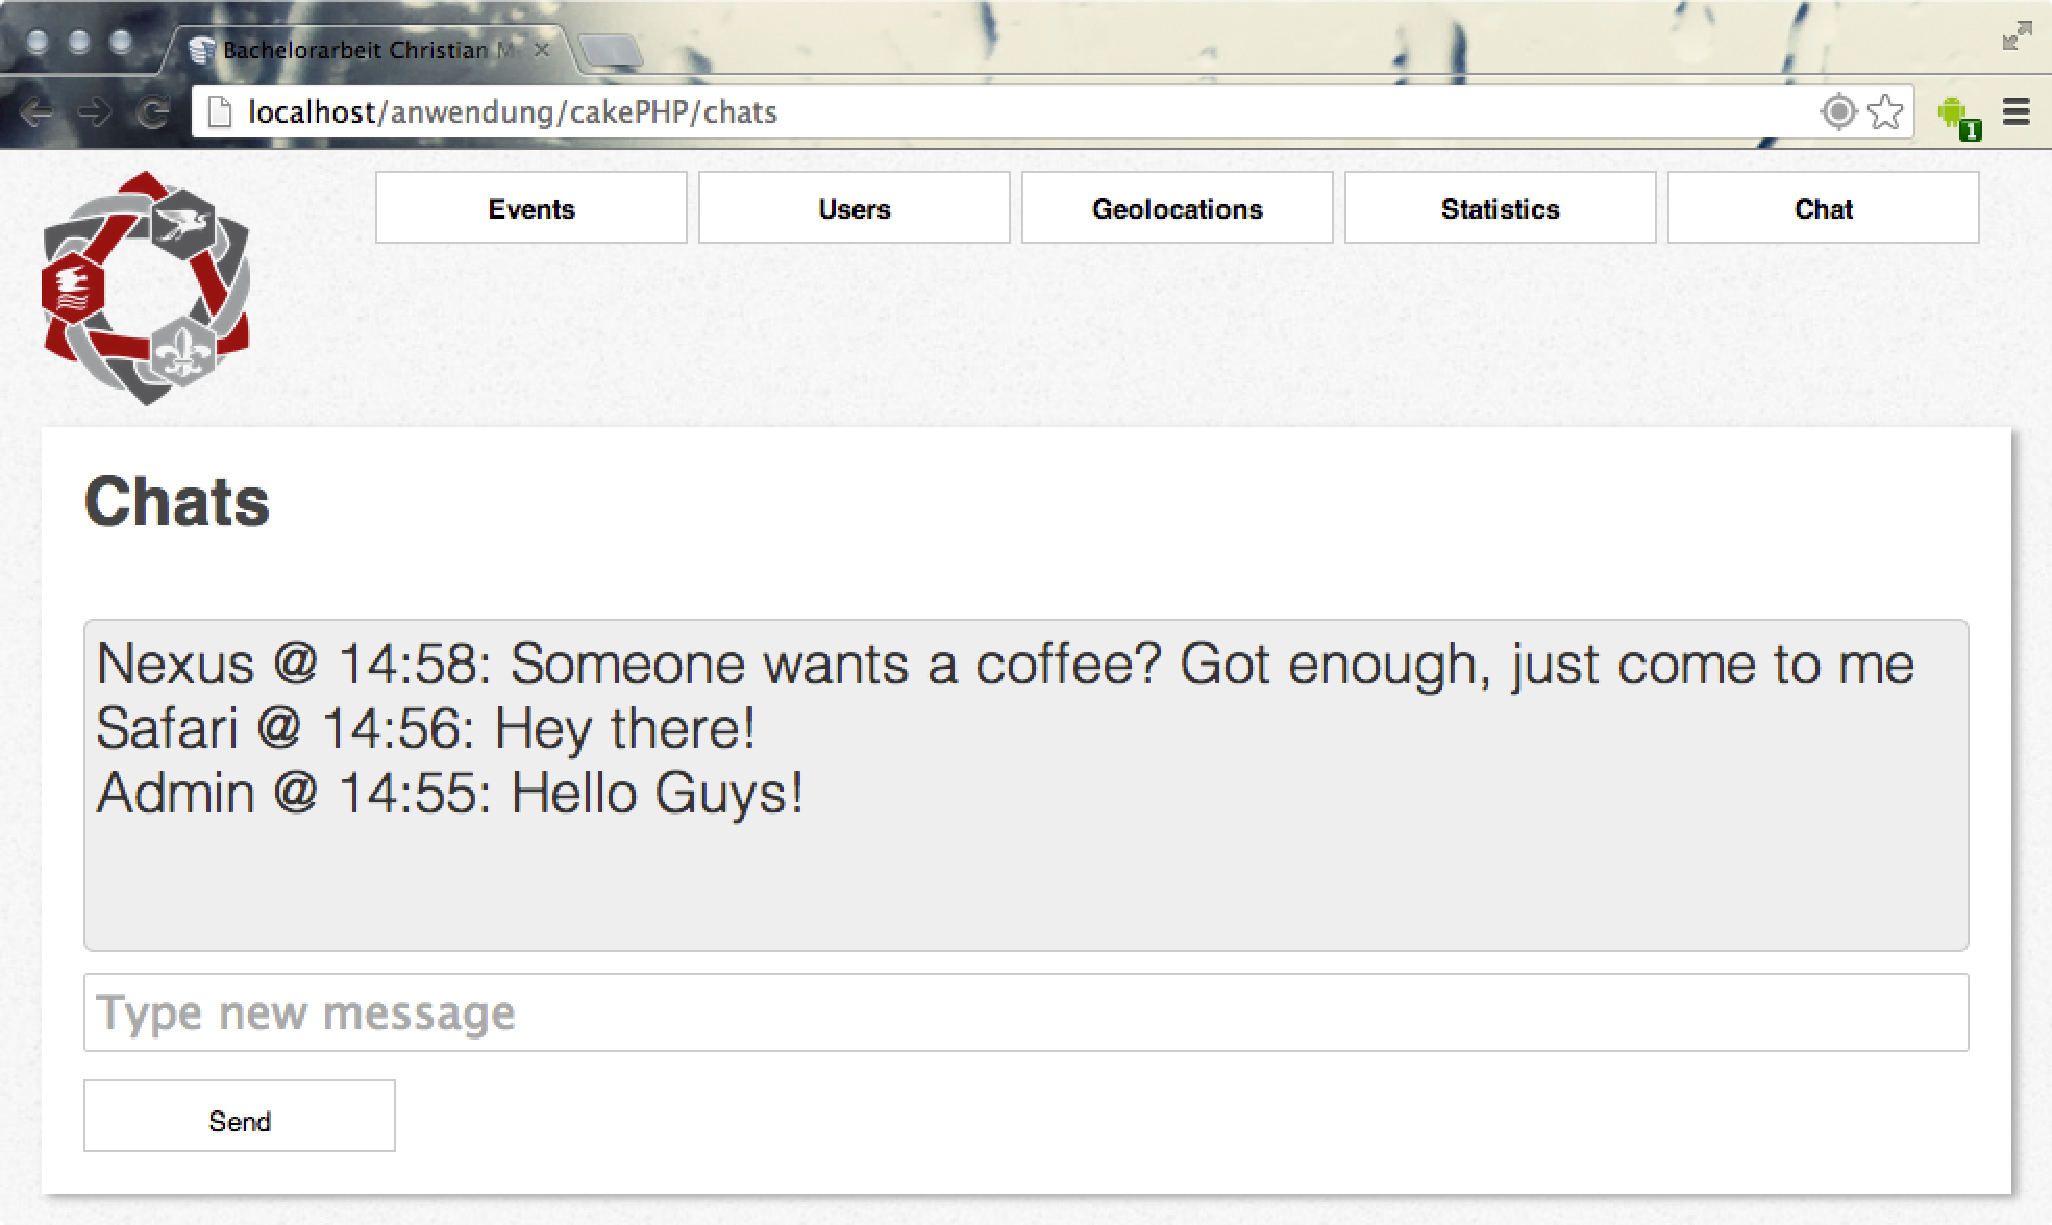
\includegraphics[width=15cm]{fig/screenshot_chat}
	\caption[Beispielansicht der Chats]{Getestet unter Chrome 29: Chatverlauf von drei verschiedenen Benutzern}
\end{figure}

Hierbei wird wieder Publish / Subscribe verwendet: Befindet sich ein Endgerät gerade im View des Chats, so abonniert die Webanwendung automatisch den Chat beim WebSocket Server und erhält dadurch alle eingehenden Nachrichten.

%%%%%%%%%%%%%%%%%%%%%%%%%%%%%%%%%%%%%%%%%%%%%%%%%%